% This is samplepaper.tex, a sample chapter demonstrating the
% LLNCS macro package for Springer Computer Science proceedings;
% Version 2.20 of 2017/10/04
%
\documentclass[runningheads]{llncs}
%
\usepackage{graphicx}
% Used for displaying a sample figure. If possible, figure files should
% be included in EPS format.
%
% If you use the hyperref package, please uncomment the following line
% to display URLs in blue roman font according to Springer's eBook style:
% \renewcommand\UrlFont{\color{blue}\rmfamily}
\usepackage{amsmath}
\usepackage{multirow}
\usepackage{makecell}
\newcommand{\argmin}{\mathop{\mathrm{arg\,min}}}

\begin{document}
%
\title{Learning Deeply Enriched Representations of Longitudinal Imaging-Genetic Data to Predict Alzheimer's Disease Progression}
%
%\titlerunning{Abbreviated paper title}
% If the paper title is too long for the running head, you can set
% an abbreviated paper title here
%
% \author{Anonymous Author(s)}
%
% \authorrunning{F. Author et al.}
% First names are abbreviated in the running head.
% If there are more than two authors, 'et al.' is used.
%
% \institute{Princeton University, Princeton NJ 08544, USA \and
% Springer Heidelberg, Tiergartenstr. 17, 69121 Heidelberg, Germany
% \email{lncs@springer.com}\\
% \url{http://www.springer.com/gp/computer-science/lncs} \and
% ABC Institute, Rupert-Karls-University Heidelberg, Heidelberg, Germany\\
% \email{\{abc,lncs\}@uni-heidelberg.de}}
%
\maketitle              % typeset the header of the contribution
%
\begin{abstract}
% The abstract should briefly summarize the contents of the paper in
% 150--250 words.
% (However, missing records that broadly exist in the longitudinal neuroimaging data have posed a critical challenge for effectively using these data in machine learning models.)
% (To tackle these difficulties, in this paper we propose a novel approach to integrate longitudinal (dynamic) phenotypic data and static genetic data to learn a fixed-length biomarker representation using the enrichment learned from the temporal data in multiple imaging modalities.)
% enriched biomarker representation, as a fixed-length vector per participant,
% We use a composite model of  autoencoders based on Recurrent Neural Network.
Alzheimer’s Disease (AD) is a progressive memory disorder that causes irreversible cognitive decline. As the early diagnosis is important to prevent AD progression, many biomarker analysis models have been presented to detect the progression in its early stage. However, these models often fail to integrate longitudinal (dynamic) phenotypic data with the static genetic data, and/or cannot deal with the missing data in the incomplete temporal neuroimaging records. To tackle these difficulties, we propose the semi-supervised enrichment learning method to learn the fixed-length vectorial representation of multi-modal data per participant. Our enrichment model is the ensemble of the novel long short-term memory (LSTM) autoencoder and the deep neural networks which is designed to handle multi-modal information and utilize the labeled and unlabeled samples both. We have applied our new method on the Alzheimer's Disease Neuroimaging Initiative (ADNI) cohort and achieved 75\% accuracy on multiclass AD progression prediction task for 1 year ahead. In addition to the improved prediction performance when compared against some widely used machine learning algorithms, our deep learning model identifies the disease relevant biomarkers.\footnote{The codes used in our experiments will be made publicly accessible on GitHub upon paper acceptance.}
% \keywords{First keyword  \and Second keyword \and Another keyword.}
\end{abstract}
% Your manuscript should be no longer than 12 pages (including references), and anonymized.

\iffalse
Mild cognitive impairment (MCI) is a transitional stage between age-related cognitive decline and Alzheimer’s disease (AD). For the effective treatment of AD, it would be important to identify MCI patients at high risk for conversion to AD. 
The novel characteristics of the methods for learning the biomarkers are as follows: 1) We used a semi-supervised learning method (low density separation) for the construction of MRI biomarker as opposed to more typical supervised methods; 2)
4) We constructed the aggregate biomarker by first learning a separate MRI biomarker and then combining it with age and cognitive measures about the MCI subjects at the baseline by applying a random forest classifier.
Alzheimer’s disease (AD), a common form of dementia, occurs most frequently in aged population. More than 30 million people worldwide suffer from AD and, due to the increasing life expectancy, this number is expected to triple by 2050 (The projected effect of risk factor reduction on Alzheimer's disease prevalence, Barnes DE).
Because of the dramatic increase in the prevalence of AD, the identification of effective biomarkers for the early diagnosis and treatment of AD in individuals at high risk to develop the disease is crucial.
Mild cognitive impairment (MCI) is a transitional stage between age-related cognitive decline and AD, and the earliest clinically detectable stage of progression towards dementia or AD (Neuropathologic alterations in mild cognitive impairment: a review, Markesbery WR). 
AD pathology has been therefore hypothesized to be detectable using neuroimaging techniques.(Neuropathologic alterations in mild cognitive impairment: a review, Markesbery WR)
Among different neuroimaging modalities, MRI has attracted a significant interest in AD related studies because of its completely non-invasive nature, high availability, high spatial resolution and good contrast between different soft tissues.
Clearly, predicting this disease in the early stages and preventing it from progressing is of great importance.
The diagnosis of Alzheimer’s disease (AD) requires a variety of medical tests, which leads to huge amounts of multivariate heterogeneous data. It can be difficult and exhausting to manually compare, visualize, and analyze this data due to the heterogeneous nature of medical tests; therefore, an efficient approach for accurate prediction of the condition of the brain through the classification of magnetic resonance imaging (MRI) images is greatly beneficial and yet very challenging. In this paper, a novel approach is proposed for the diagnosis of very early stages of AD through an efficient classification of brain MRI images
Next, using a small set of labeled training data,
The reason that early diagnosis of AD is of great importance is that the clinical therapies given to patients are much more effective in slowing down disease progression and helping preserve some cognitive functions of the brain if the patients are in the early stages of their disease.
In this paper, we propose a novel method for a high-level latent and shared feature representation from neuroimaging modalities via deep learning. 
Furthermore, fusing the complementary information from multiple modalities helps enhance the diagnostic accuracy[Identification of conversion from mild cognitive impairment to Alzheimer's disease using multivariate predictors.; Multivariate examination of brain abnormality using both structural and functional MRI.]
To this end, many researchers have devoted their efforts to find biomarkers and develop a computer-aided system, with which we can effectively predict or diagnose the diseases.
In a semi-supervised method, feature vectors from unlabeled data are also used in the learning process in addition to the labels and feature vectors from the labeled ones.
\fi

\section{Introduction}
% Why our model is good? : (1) Semi-supervised learning -> Our model can learn from labeled/unlabeled samples BOTH. (2) Learn temporal trends from the time series with missing records (MRI imagings are captured inconsistently (the number of records/the time points of records are different) from the participants). (3) Combine the multi-modal (genotypic modality (SNPs, static) + phenotypic (neuroimagings, dynamic) modality) data with two Autoencoders: one for static, another for time series.
% Find the related works with the lack of above advantages of our model.
\iffalse
For AD progression prediction using longitudinal phenotypic markers, the input imaging features are a set of matrices X = {X1, X2, . . . , XT } ∈ Rd×n×T corresponding to the measurements at T consecutive time points, where Xt is the phenotypic measurements for a certain type of imaging markers, such as voxel-based morphometry (VBM) markers (see details in Section 3) used in this study, at time t (1 ≤ t ≤ T ).
\fi

\section{The Dataset and Problem Formalization}
\subsection{Datasets}
We obtained the data used in this experiment from the ADNI database~\cite{risacher2010longitudinal}. We downloaded 1.5 T MRI scans, single nucleotide polymorphisms (SNPs), and demographic information (age and gender) of 821 ADNI-1 participants. For the SNPs data, the quality control steps discussed in~\cite{shen2010whole} were followed, and 1223 SNPs for each participant are extracted. We performed voxel-based morphometry (VBM) and FreeSurfer (FS) on the MRI data following~\cite{risacher2010longitudinal} and extracted mean modulated gray matter measures for 90 target regions of interest. We also downloaded the longitudinal scores of the participants in five independent cognitive assessments including Alzheimer’s Disease Assessment Scale (ADAS), Mini-Mental State Examination (MMSE), Fluency test (FLU), Rey’s Auditory Verbal Learning Test (RAVLT) and Trail making test (TRAILS). 
% We also downloaded the longitudinal scores of the participants in five independent cognitive assessments including Alzheimer’s Disease Assessment Scale (ADAS)~\cite{rosen1984new}, Mini-Mental State Examination (MMSE)~\cite{tombaugh1992mini}, Fluency test (FLU)~\cite{ruff1987ruff}, Rey’s Auditory Verbal Learning Test (RAVLT)~\cite{moradi2017rey} and Trail making test (TRAILS)~\cite{reitan1958validity}. 
% Details about these cognitive assessments are available in the ADNI procedure manuals\footnote{http://adni.loni.usc.edu/wp-content/uploads/2010/09/ADNI\_GeneralProceduresManual.pdf}. 
In this analysis, the time points for both imaging records and cognitive assessments include baseline (BL), month 6 (M6), month 12 (M12), month 18 (M18), and month 24 (M24). We use the diagnosis at month 36 (M36) in Alzheimer's disease (AD), mild cognitive impairment (MCI), and healthy control(HC) as predictive target in our studies. The participants with no missing SNPs, demographic information, and AD diagnosis at M36 were included, providing a set of 379 subjects (104 AD, 115 MCI, 160 HC). The studied cohort includes 231 male and 148 female participants, and the average age is 75.35.
% Why multi class?

In the following pages, we denote a vector as a bold lower case letter, and a matrix as a bold upper case letter. For the arbitrary matrix $\mathbf{X}$, $[\mathbf{X}]^r$, $[\mathbf{X}]_c$, $[\mathbf{X}]^r_c$ denotes the $r$-th row, $c$-th column, an element of $r$-th row and $c$-th column respectively. We use $i$ and $j$ to index the participant and record respectively. We describe the records of the $i$-th participant as $\mathcal{X}_i = \{\mathbf{x}_i^b, \mathbf{x}_i^s, \mathbf{X}_i, \mathbf{M}_i, \mathbf{t}_i\}$. $\mathbf{x}_i^b \in \Re^{D_b}$ is a vector of basic demographic information (age and gender, $D_b = 2$), $\mathbf{x}_i^s \in \Re^{D_s}$ is a vector of SNPs ($D_s = 1223$), and $\mathbf{X}_i = [\mathbf{x}_i^1; \mathbf{x}_i^2; \cdots; \mathbf{x}_i^{n_i}] \in \Re^{n_i \times D_l}$ are the longitudinal records collected across the $n_i$ time points. $\mathbf{M}_i = [\mathbf{m}_i^1; \mathbf{m}_i^2; \cdots; \mathbf{m}_i^{n_i}] \in \{1, 0\}^{n_i \times D_l}$ are the binary masks of longitudinal records $\mathbf{X}_i$, where 1 and 0 indicates the observed and unobserved entry. Each longitudinal record at the $j$-th time point $\mathbf{x}_i^j$ ($1 \leq j \leq n_i$) is the concatenation of multi-modal neuroimagings and cognitive assessments, such that $\mathbf{x}_i^j = $ $[\mathbf{x}_{i,VBM}^j$, $\mathbf{x}_{i,FS}^j,$ $\mathbf{x}_{i,ADAS}^j,$ $\mathbf{x}_{i,MMSE}^j,$ $\mathbf{x}_{i,FLU}^j,$ $\mathbf{x}_{i,RAVLT}^j,$ $\mathbf{x}_{i,TRAILS}^j] \in \Re^{D_l}$, and the missing records are filled with the constant $-1$. $\mathbf{t}_i = [t_i^1; t_i^2; \cdots; t_i^{n_i}] \in \Re^{n_i}$ are the time stamps of $n_i$ records. The target label $\mathbf{y}_i \in \Re^{D_y}$ of the $i$-th participant is given for training if that participant is in training set, such that $i \in \Omega_{train}$. 
% The target label is one-hot encoded, such that $[1, 0, 0]$, $[0, 1, 0]$, and $[0, 0, 1]$ represent AD, MCI, and HC respectively. 
The input and output of the proposed model is described in Fig.~\ref{fig: final-inputs}.
\begin{figure}
    \centering
    \includegraphics[width=0.95\textwidth]{images/final-inputs.png}
    \caption{Armed with the enriched representations of dynamic and static data, we can fully utilize the information in the dataset. 
    % The demographic information is provided without enrichment, as it's dimensionality is relatively small.
    } \label{fig: final-inputs}
\end{figure}

\subsection{Enrichment and Objective Formulation}
\subsubsection{Static Data Enrichment}
We leverage the autoencoder~\cite{kramer1991nonlinear} to learn the enriched representation of genotypic biomarkers. The autoencoder consists of two deep neural networks: an encoder $\phi_{SNP}: \Re^{D_s} \mapsto \Re^{d_s}$ that encodes a vector of SNPs into the enriched representation such that $\phi_{SNP}(\mathbf{x}_i^s;\ \theta^s_{E}) = \mathbf{z}_i^s$, and an decoder $\psi_{SNP}: \Re^{d_s} \mapsto \Re^{D_s}$ that decodes the enriched representation into the reconstructed vector of SNPs such that $\psi_{SNP}(\mathbf{z}_i^s;\ \theta^s_{D}) = \tilde{\mathbf{x}}_i^s$. $\theta_{E}^s$ and $\theta_{D}^s$ is the set of trainable weights matrices and bias vectors for the encoder and decoder respectively. 
% The deep neural network is defined as the $K$ consecutive fully connected layers where the output of the $k$-th layer is:
% \begin{equation}
%     \mathbf{h}_k = \sigma(\mathbf{h}_{k-1}\mathbf{W}_k + \mathbf{b}_k),
% \end{equation}
% where $\sigma$ is an activation function.
% The input $\mathbf{h}_0$ of the network is then forwarded to the last layer $\mathbf{h}_K = \tilde{\mathbf{x}}_i^s$, which is the output of the network. 
The encoded representation $\mathbf{z}_i^s$ preserves as much information as possible while removing the redundant noises in SNPs $\mathbf{x}_i^s$ by updating $\theta_{E}^s$ or $\theta_{D}^s$ to minimize the following reconstruction loss:
\begin{equation}
    \mathcal{L}_{static}(\mathbf{x}_i^s, \tilde{\mathbf{x}}_i^s;\ \theta_{E}^s, \theta_{D}^s) = \left\|\mathbf{x}_i^s - \tilde{\mathbf{x}}_i^s\right\|_F^2,
\end{equation}
where squared Frobenious norm $\| \cdot \|_F^2$ is summation of all the entries squared.

% then combining it with age and cognitive measures.
% Our models summarizes the dynamic and static data into a fixed-length vectorial representation.
% We use Long Short Term Memory (LSTM) architecture to learn the fixed-length vectorial abstract representation summarizing the incomplete time series with varying length and uneven time intervals.
% [In this section, we describe the semi-supervised AutoEncoder (AE) structure to learn a fixed-length vectorial representation for each patient's longitudinal records with varying length. The proposed AE is a composite model of three components. The encoder $\phi_E$ learns an abstract enriched representation of the input time series data. The decoder $\phi_D$ learns the reconstruction system to estimate the original data from the enriched representation. The predictor $\phi_P$ learns the prediction system to estimate the target labels from the enriched representation.].

\subsubsection{Dynamic Data Enrichment}
LSTM encoder $\phi_{dynamic}: \Re^{n_i \times (2 D_l + 1)} \mapsto \Re^{d_l}$ summarizes the longitudinal records $\mathbf{X}_i$ in the fixed-length vector $\mathbf{z}_i^l$. The time stamp of each record is crucial in learning the temporal relation (e.g. temporal locality) between records, and the pattern of missing entries may help the encoder to interpret the input. Thus we provide the concatenation of longitudinal records, masks, and time stamps, $[\mathbf{X}_i, \mathbf{M}_i, \mathbf{t}_i] = [\hat{\mathbf{x}}_i^1; \hat{\mathbf{x}}_i^2; \cdots; \hat{\mathbf{x}}_i^{n_i}] = \hat{\mathbf{X}}_i \in \Re^{n_i \times (2 D_l + 1)}$, as an input of the LSTM encoder such that $\phi_{dynamic}(\mathbf{X}_i, \mathbf{M}_i, \mathbf{t}_i;\ \theta_{E}^l) = \mathbf{z}_i^l$. 

The concatenated longitudinal record at the $j$-th time step $\hat{\mathbf{x}}_i^j$ ($1 \leq j \leq n_i$) is processed by the following LSTM architecture~\cite{yu2019review}:
\begin{equation}
    \mathbf{k}^j_i = \sigma(\hat{\mathbf{x}}^j_i \mathbf{W}_{xk} + \mathbf{h}_i^{j-1} \mathbf{W}_{hk} + \mathbf{c}_i^{j-1} \mathbf{W}_{ck} + \mathbf{b}_k),
\end{equation}
\begin{equation}
    \mathbf{f}^j_i = \sigma(\hat{\mathbf{x}}^j_i \mathbf{W}_{xf} + \mathbf{h}^{j-1}_i \mathbf{W}_{hf} + \mathbf{c}^{j-1}_i \mathbf{W}_{cf} + \mathbf{b}_f),
\end{equation}
\begin{equation}
    \mathbf{c}^j_i = \mathbf{f}^j_i \odot \mathbf{c}^{j-1}_i + \mathbf{k}^j_i \odot \operatorname{tanh}(\hat{\mathbf{x}}_i^j \mathbf{W}_{xc} + \mathbf{h}^{j - 1}_i \mathbf{W}_{hc} + \mathbf{b}_c),
\end{equation}
\begin{equation}
    \mathbf{o}^j_i = \sigma(\hat{\mathbf{x}}_i^j \mathbf{W}_{xo} + \mathbf{h}^{j-1}_i \mathbf{W}_{ho} + \mathbf{c}^j_i \mathbf{W}_{co} + \mathbf{b}_o),
\end{equation}
\begin{equation}
    \mathbf{h}^j_i = \mathbf{o}^j_i \odot \operatorname{tanh}(\mathbf{c}^j_i),
\end{equation}
% \begin{equation}
% \begin{aligned}
%     \mathbf{k}^j_i = \sigma(\hat{\mathbf{x}}^j_i \mathbf{W}_{xk} + \mathbf{h}_i^{j-1} \mathbf{W}_{hk} + \mathbf{c}_i^{j-1} \mathbf{W}_{ck} + \mathbf{b}_k),\ \mathbf{f}^j_i = \sigma(\hat{\mathbf{x}}^j_i \mathbf{W}_{xf} + \mathbf{h}^{j-1}_i \mathbf{W}_{hf} + \mathbf{c}^{j-1}_i \mathbf{W}_{cf} + \mathbf{b}_f),
% \end{aligned}
% \end{equation}
where $\mathbf{k}^j_i$, $\mathbf{o}^j_i$, $\mathbf{f}^j_i$ are the input, output, and forget gate of the $j$-th time step respectively. \{$\mathbf{W}_{xk}$, $\mathbf{W}_{hk}$, $\mathbf{W}_{ck}$, $\mathbf{W}_{xf}$, $\mathbf{W}_{hf}$, $\mathbf{W}_{cf}$, $\mathbf{W}_{xc}$, $\mathbf{W}_{hc}$, $\mathbf{W}_{xo}$, $\mathbf{W}_{ho}$, $\mathbf{W}_{co}$\} $\subset \mathbf{\theta}_{E}^l$ are trainable weight matrices and $\{\mathbf{b}_k, \mathbf{b}_f, \mathbf{b}_c, \mathbf{b}_o\} \subset \mathbf{\theta}_{E}^l$ are trainable bias vectors. $\mathbf{c}_i^j$ and $\mathbf{h}_i^j$ denote the cell state and hidden representation. The hidden representation $\mathbf{h}_i^{n_i}$ at the last time step $n_i$ represents a summary of \emph{whole} longitudinal records $\hat{\mathbf{X}}_i$, such that $\mathbf{h}_i^{n_i} = \mathbf{z}_i^l \in \Re^{d_l}$. Since the hidden representation at the $j$-th time point aims to summarize the records from the first time step to the $j$-th time step, it refers to the cell state $\mathbf{c}_i^j$ containing information about the previous records. The cell state $\mathbf{c}_i^j$ is guided by the input gate $\mathbf{k}_i^j$ and forget gate $\mathbf{f}_i^j$, which control how much information from the previous step should be preserved, therefore cell state $\mathbf{c}_i^j$ enables the hidden representation $\mathbf{h}_i^j$ to learn long term dependencies. 
% For example, the LSTM encoder can capture the cognitive decline from the temporal trends in the scores of cognitive assessments.

% (RNN)~\cite{medsker2001recurrent}
We propose a decoder for dynamic data enrichment with a fully connected layers instead of another LSTM. A previous study~\cite{srivastava2015unsupervised} that attempted to enrich longitudinal records with a recurrent neural network, did so by using RNNs for both the encoder and decoder, where the output (reconstructed record) of the decoder at each time step depends on the output at the previous time step. However, since no additional information is provided to the decoder other than a time stamp and a learned representation that is no longer longitudinal, there should not be dependency between the outputs of the decoder. Therefore the decoder $\psi_{dynamic}:\Re^{d_l + 1} \mapsto \Re^{D_l}$ should be able to reconstruct the $j$-th record $\mathbf{x}_i^j$ given time stamp $t_i^j$ without any additional information, such that $\psi_{dynamic}(\mathbf{z}_i^l, t^j_i;\ \theta^l_{D}) = \tilde{\mathbf{x}}_i^j \approx \mathbf{x}_i^j$. This architecture, to the best of our knowledge, has not yet been proposed. We update $\theta^l_{E}$ and $\theta^l_{D}$ to minimize the error between the reconstructed and original records for the observed entries defined as: 
% indicated by the mask $\mathbf{M}_i$:
\begin{equation}
    \mathcal{L}_{dynamic}(\mathbf{X}_i, \tilde{\mathbf{X}}_i, \mathbf{M}_i;\ 
    \theta^l_{E}, \theta^l_{D}) = \frac{\left\| (\tilde{\mathbf{X}}_i
- \mathbf{X}_i) \odot \mathbf{M}_i
\right\|_F^2}{\sum_{q=1}^{D_l}\sum_{j=1}^{n_i}[\mathbf{M}_i]^j_q},
\end{equation}
where $\tilde{\mathbf{X}}_i \in \Re^{n_i \times D_l}$ is the stack of reconstructed $n_i$ records of $i$-th participant. 
% Why decoder is not RNN? Think of what is input for encoder and decoder. Because there is no information is additionally provided, current prediction depends on previous prediction does not make sense. The enriched representation is the fixed-length vector which is not longitudinal records anymore.

% Although the enriched representation is learned from a few of observations, it represents the whole temporal dimension of timeseries.
% Given the enriched representation $\mathbf{z}_i^l$, the decoder tries to estimate the function of time $\psi_{dynamic}(t; \mathbf{z}_i^l)$ to reconstruct the state of biomarker representation in temporal dimension.

\subsubsection{Prediction and Loss Function}
From the enriched representations $\mathbf{z}_i^l$ and $\mathbf{z}_i^s$ of dynamic and static data, another fully connected layer $\psi_{pred}: \Re^{(d_s + d_l + D_b)}  \mapsto \Re^{D_y}$ predicts the target label $\mathbf{y}_i$, such that $\psi_{pred}(\mathbf{z}_i^l, \mathbf{z}_i^s, \mathbf{x}_i^b;\ \theta_{D}^p) = \tilde{\mathbf{y}}_i$.
We design the loss function inducing the enriched representation to convey the useful information to reconstruct the original records and predict the target label:
\begin{equation}\label{eq: total loss}
\begin{aligned}
    &\theta_{E}^s, \theta_{D}^s, \theta^l_{E}, \theta^l_{D}, \theta^p = \argmin_{\theta_{E}^s, \theta_{D}^s, \theta^l_{E}, \theta^l_{D}, \theta^p} \bigl(\gamma_1 \mathcal{L}_{predict}(\mathbf{y}_i, \tilde{\mathbf{y}}_i;\ \theta^p) \\
    & + \gamma_2 \mathcal{L}_{static}(\mathbf{x}_i^s, \tilde{\mathbf{x}}_i^s;\ \theta_{E}^s, \theta_{D}^s) + \gamma_3 \mathcal{L}_{dynamic}(\mathbf{X}_i, \tilde{\mathbf{X}}_i, \mathbf{M}_i;\ \theta^l_{E}, \theta^l_{D})\bigr),
\end{aligned}
\end{equation}
where $\gamma_1$, $\gamma_2$, and $\gamma_3$ are hyperparameters to adjust the impact of each loss. 
We choose the cross entropy for the prediction loss defined as follows:
\[
\mathcal{L}_{predict}\bigl(\mathbf{y}_i, \tilde{\mathbf{y}}_i;\ \theta_{D}^p\bigr)=
\begin{cases}
0 & i \notin \Omega_{train},\\
- \left\|\mathbf{y}_i \odot \operatorname{log}(\tilde{\mathbf{y}}_i) + (\mathbf{1} - \mathbf{y}_i) \odot \operatorname{log}(\mathbf{1} - \tilde{\mathbf{y}}_i)\right\|_1 & i \in \Omega_{train},
\end{cases}
\]
where $\mathbf{1}$ is a vector of 1's and $\operatorname{log}$ is an element-wise logarithm function. The illustration of loss function is provided in supplementary.

\iffalse
Data used in this work include all subjects for whom baseline MRI data (T1-weighted MP-RAGE sequence at 1.5 T, typically 256 × 256 × 170 voxels with the voxel size of approximately 1 mm × 1 mm × 1.2 mm), at least moderately confident diagnoses (i.e. confidence > 2), hippocampus volumes (i.e. volumes of left and right hippocampi, calculated by FreeSurfer Version 4.3), and test scores in certain cognitive scales (i.e. ADAS: Alzheimer’s Disease Assessment Scale, range 0–85; CDR-SB: Clinical Dementia Rating ‘sum of boxes’, range 0–18; MMSE: Mini-Mental State Examination, range 0–30) were available.
Because one of the primary goals of our regression analysis is to identify a subset of imaging markers which are highly correlated to the AD progression reflected by the cognitive changes over time.
In summary, the identified longitudinally stable imaging markers are highly suggestive and strongly agree with the existing research findings,

The time points examined in this study for both imaging biomarkers and cognitive assessments include the baseline (BL), the 6th month (M6), the 12th month (M12), the 18th month (M18), the 24th month (M24) and the 36th month (M36).

As a result, a total of 544 sample subjects are selected in our study, among which 92 samples are diagnosed with AD, 205 samples are diagnosed to be with Mild Cognitive Impairment (MCI), and 177 samples are HC.

From the top panel of Fig. 4 we can see that the VBM biomarkers with highest weights are perfectly in accordance with existing medical findings. Specifically, we observe that the bilateral hippocampus are among the top selected biomarkers. In addition, the bilateral amygdala is also among the top selected biomarkers. Finally, We notice that the bilateral putamen are also among the top selected biomarkers. , which is one more indication of the correctness our new method.
Specifically, if the number of labeled images is small, semi-supervised approach appears to yield higher classification accuracy.
\fi

\section{Experiments} % 3.5 pages length recommended.
% The distribution of a feature may be categorized -> swap is better than gradient.
Our experiments consist of two parts: (1) we compare the prediction performance of the proposed model to the widely used prediction models, and (2) we identify the biomarkers which are most predictive for AD progression.
% We use AD progression in AD, MCI and HC as predictive targets in our studies.
% Although their deep learning approaches have shown the promising prediction results in binary classifications, but multi-class models have not achieved enough accuracy for clinical applicability.
\subsection{Classification Performance}
\subsubsection{Competing models}
For an ablation study to observe the effectiveness of our semi-supervised autoencoder (SAE), we introduce a baseline LSTM (BLSTM) model by removing decoders $\psi_{SNP}$ and $\psi_{dynamic}$ from our model SAE. In addition to the longitudinal model, we use the random forest~\cite{ho1995random} (RF) with 34 max depth and deep neural network (DNN) with 5 fully connected layers. Since these competing models are not longitudinal, we provide the concatenation of the most recent record $[\mathbf{x}_i^b, \mathbf{x}_i^s, \mathbf{x}_i^{n_i}]$ to them. Both the training and test sets are provided to train SAE in a semi-supervised manner, while the other competing models are trained only with the training set. Although the order of participants is randomly shuffled to avoid the bias, we use the same training and test data across all the competing methods for a fair comparison. The hyperparameters of our model are provided in the supplementary.
\subsubsection{Result and Evaluation}
We conduct the multiclass AD progression prediction task for 1 year ahead.
% \begin{equation}\label{eq: metrics}
% \begin{aligned}
%     &\text{Accuracy} = \frac{\sum_{c \in C}(TP_c + TN_c)}{\sum_{c \in C}(TP_c + TN_c + FP_c + FN_c)},\\
%     &\text{Precision of class }c=\frac{TP_c}{TP_c + FP_c},\ \text{Recall of class }c=\frac{TP_c}{TP_c+FN_c},
% \end{aligned}
% \end{equation}
% where $C$ is a set of classes \{AD, MCI, HC\}.
In table~\ref{tab: experimetal results}, the average and standard deviation of performance results across $k$ groups are reported following a $k$-fold cross validation scheme. We split the dataset into $k=2,\ 3,\ 5$ subgroups, such that 50\%, 66\%, 80\% of participants belong to the training set respectively. In table~\ref{tab: experimetal results}, nan (not a number) in precision on specific class means the model never predicted that class in one of $k$ subgroups.
% Considering the prediction of random forest is biased towards AD (high AD Recall), our model SAE generally outperforms other competing models. Interestingly, the performance gap between SAE and BLSTM increases as the size of training set decreases. 
Our model SAE generally outperforms other competing models especially when the proportion of training set is small. We suppose that this is because our semi-supervised learning approach can learn from the unlabeled samples in test set, while the other models cannot. This finding shows our model's promise in the early diagnosis of AD.
% This finding shows our model's versatility in handling samples, as well as its promise in the early diagnosis of AD.
% [Emphasize AD precision, recall as it is good, and important to detect than MCI and HC, can detect characteristics of the samples of AD participant.]

\begin{table*}[ht]
    \centering
    \caption{The prediction performance from k-fold cross validation. Receiver operating characteristic curves of this result is provided in supplementary.}\label{tab: experimetal results}
    \begin{tabular}{c c cccc}
        \toprule
    \multirow{1}{*}{\bfseries Training Set} & {\bfseries Metric} & \multicolumn{1}{c}{{\bfseries SAE} (Ours)} & \multicolumn{1}{c}{{\bfseries BLSTM}} & \multicolumn{1}{c}{{\bfseries RF}} & {\bfseries DNN}         \\
    \midrule
    \multirow{7}{*}{80\%} %% 7 rows group.
    & Accuracy & \multicolumn{1}{c}{{\bfseries 74.95$\pm$4.72}} & \multicolumn{1}{c}{71.57$\pm$5.29} & \multicolumn{1}{c}{71.79$\pm$6.33} & 49.45$\pm$2.91\\
    & AD Precision & \multicolumn{1}{c}{{\bfseries 71.28$\pm$11.89}} & \multicolumn{1}{c}{71.19$\pm$16.79} & \multicolumn{1}{c}{70.55$\pm$9.22} & 55.13$\pm$6.30\\
    & MCI Precision & \multicolumn{1}{c}{59.84$\pm$10.11} & \multicolumn{1}{c}{{\bfseries 60.07$\pm$11.74}} & \multicolumn{1}{c}{59.64$\pm$8.15} & 33.84$\pm$4.97\\
    & HC Precision & \multicolumn{1}{c}{{\bfseries 89.69$\pm$7.33}} & \multicolumn{1}{c}{86.60$\pm$8.15} & \multicolumn{1}{c}{87.28$\pm$9.88} & 47.02$\pm$7.9\\
    & AD Recall & \multicolumn{1}{c}{69.30$\pm$7.30} & \multicolumn{1}{c}{65.92$\pm$21.31} & \multicolumn{1}{c}{{\bfseries 71.18$\pm$12.64}} & 74.49$\pm$7.45\\
    & MCI Recall & \multicolumn{1}{c}{{\bfseries 66.00$\pm$11.83}} & \multicolumn{1}{c}{60.00$\pm$8.57} & \multicolumn{1}{c}{61.47$\pm$11.93} & 22.89$\pm$2.93\\
    & HC Recall & \multicolumn{1}{c}{85.36$\pm$8.98} & \multicolumn{1}{c}{{\bfseries 89.37$\pm$6.53}} & \multicolumn{1}{c}{86.58$\pm$9.50} & 36.33$\pm$8.67\\
    \midrule
    \multirow{7}{*}{66\%} %% 7 rows group.
    & Accuracy & \multicolumn{1}{c}{{\bfseries 73.34$\pm$1.71}} & \multicolumn{1}{c}{69.92$\pm$1.94} & \multicolumn{1}{c}{61.83$\pm$4.02} & 47.81$\pm$1.65\\
    & AD Precision & \multicolumn{1}{c}{{\bfseries 63.47$\pm$7.84}} & \multicolumn{1}{c}{62.10$\pm$5.53} & \multicolumn{1}{c}{51.63$\pm$1.29} & 55.26$\pm$1.61\\
    & MCI Precision & \multicolumn{1}{c}{{\bfseries 63.97$\pm$8.74}} & \multicolumn{1}{c}{55.39$\pm$7.85} & \multicolumn{1}{c}{53.91$\pm$8.85} & 31.03$\pm$1.37\\
    & HC Precision & \multicolumn{1}{c}{{\bfseries 88.62$\pm$3.47}} & \multicolumn{1}{c}{85.94$\pm$3.09} & \multicolumn{1}{c}{71.74$\pm$3.14} & 46.64$\pm$6.77\\
    & AD Recall & \multicolumn{1}{c}{{\bfseries 69.14$\pm$6.16}} & \multicolumn{1}{c}{63.90$\pm$7.23} & \multicolumn{1}{c}{59.48$\pm$8.8} & 70.09$\pm$6.63\\
    & MCI Recall & \multicolumn{1}{c}{{\bfseries 56.97$\pm$8.32}} & \multicolumn{1}{c}{53.85$\pm$10.16} & \multicolumn{1}{c}{39.09$\pm$11.54} & 27.62$\pm$5.09\\
    & HC Recall & \multicolumn{1}{c}{{\bfseries 88.55$\pm$3.44}} & \multicolumn{1}{c}{85.48$\pm$3.04} & \multicolumn{1}{c}{36.56$\pm$2.84} & 32.44$\pm$6.52\\
    \midrule
    \multirow{7}{*}{50\%} %% 7 rows group.
    & Accuracy & \multicolumn{1}{c}{{\bfseries 72.29$\pm$2.44}} & \multicolumn{1}{c}{47.29$\pm$23.60} & \multicolumn{1}{c}{53.69$\pm$2.04} & 47.68$\pm$0.13\\
    & AD Precision & \multicolumn{1}{c}{{\bfseries 60.79$\pm$2.25}} & \multicolumn{1}{c}{50.38$\pm$26.69} & \multicolumn{1}{c}{51.56$\pm$2.68} & 52.87$\pm$2.26\\
    & MCI Precision & \multicolumn{1}{c}{{\bfseries 60.93$\pm$6.38}} & \multicolumn{1}{c}{nan$\pm$nan} & \multicolumn{1}{c}{nan$\pm$nan} & 33.12$\pm$6.56\\
    & HC Precision & \multicolumn{1}{c}{{\bfseries 86.99$\pm$2.20}} & \multicolumn{1}{c}{nan$\pm$nan} & \multicolumn{1}{c}{64.99$\pm$2.28} & 44.38$\pm$0.06\\
    & AD Recall & \multicolumn{1}{c}{72.90$\pm$8.45} & \multicolumn{1}{c}{81.36$\pm$18.64} & \multicolumn{1}{c}{{\bfseries 98.14$\pm$0.08}} & 75.56$\pm$5.73\\
    & MCI Recall & \multicolumn{1}{c}{{\bfseries 45.21$\pm$11.24}} & \multicolumn{1}{c}{30.19$\pm$30.18} & \multicolumn{1}{c}{0.53$\pm$0.53} & 20.51$\pm$2.42\\
    & HC Recall & \multicolumn{1}{c}{{\bfseries 89.85$\pm$4.13}} & \multicolumn{1}{c}{42.21$\pm$42.20} & \multicolumn{1}{c}{36.10$\pm$0.17} & 30.70$\pm$7.16\\
        \bottomrule
    \end{tabular}
\end{table*}

\subsection{AD Relevant Biomarkers Identification}
\begin{figure}
    \centering
    \includegraphics[width=0.42\textwidth]{images/biomarker-identification/fs.png}
    \includegraphics[width=0.42\textwidth]{images/biomarker-identification/vbm.png}
    \caption{Importance distribution over the brain regions. The darker color indicates the greater importance. The top five most important regions identified are {\bf FS:} Right Lateral Ventricle, Left Para-Hippocampal, Left Amygdala, Left Cerebral White Matter, Left Hippocampus, and {\bf VBM:} Left Para-Hippocampal, Left Amygdala, Left Hippocampus, Right Hippocampus, Right Amygdala.}
    \label{fig: brain map}
\end{figure}
\begin{figure}
    \centering
    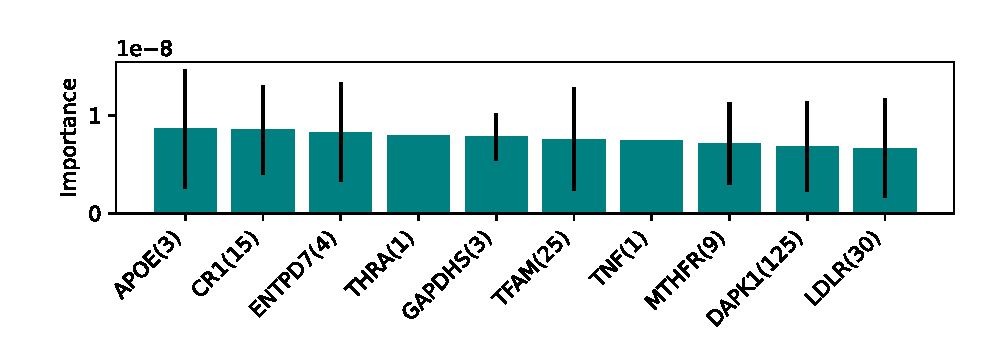
\includegraphics[width=0.85\textwidth]{images/biomarker-identification/alzgene-same-color.eps}
    \caption{Importance of each AlzGene group. The standard deviation and number of SNPs in each group is denoted by the line and the number next to the group name}\label{fig: AlzGene}
\end{figure}
% [Because of the dramatic increase in the prevalence of AD, the identification of effective biomarkers for the early diagnosis and treatment of AD in individuals at high risk to develop the disease is crucial.]
It is vital to identify AD relevant biomarkers for early detection and the treatment of people at high risk of developing AD. Despite the promising performance of deep neural networks, their predictions are notoriously difficult to interpret. To identify which biomarkers largely affect the predictions, we add the perturbation to the input data and observe the changes in prediction. The details of this identification method is described in supplementary. In Fig~\ref{fig: brain map} and Fig~\ref{fig: AlzGene}, we plot the importance distribution over the brain regions and AlzGene groups of SNPs. The AlzGene groups of SNPs have been constructed by the multiple genome-wide association studies listed on the website (\url{http://www.alzgene.org/}). From our model SAE, ventricular~\cite{carmichael2007ventricular}, hippocampus~\cite{mu2011adult}, and amygdala~\cite{poulin2011amygdala} are identified as important brain regions, and apolipoprotein E~\cite{kim2009role} and complement receptor 1~\cite{lambert2009genome} are identified as important AlzGene groups. The identified biomarkers have been shown in the literature to be related to AD, thus they provide substantial evidence that our approach can identify the biomarkers associated with AD.

% \begin{equation}\label{eq: SNPs identification}
% \begin{aligned}
%     &(\mathbf{x}_i^s)' = [x_{i, 1}^s, x_{i, 2}^s, \cdots, x_{i, m}^s + p_{i, m}, \cdots, x_{i, D_s}^s],\\
%     &\Delta\tilde{\mathbf{y}}_i = \| \psi_{pred}\bigl(\phi_{dynamic}(\mathbf{X}_i, \mathbf{M}_i, \mathbf{t}_i;\ \theta_{\phi}^d),\ \psi_{SNP}(\phi_{SNP}((\mathbf{x}_i^s)';\ \theta^s_{\phi});\ \theta^s_{\psi}),\ \mathbf{x}_i^b;\ \theta^p_{\psi}\bigr)\\
%     &- \psi_{pred}\bigl(\phi_{dynamic}(\mathbf{X}_i, \mathbf{M}_i, \mathbf{t}_i;\ \theta_{\phi}^d),\ \psi_{SNP}(\phi_{SNP}(\mathbf{x}_i^s;\ \theta^s_{\phi});\ \theta^s_{\psi}),\ \mathbf{x}_i^b;\ \theta^p_{\psi}\bigr)\|_1.
% \end{aligned}
% \end{equation}
% Finally, we plot top 15 most important features in Fig..
% \subsubsection{AD relevant imaging biomarkers}
% In Fig~\ref{fig: brain map}, we plot the importance distribution over the brain regions.
% % calculated by Eq.~\eqref{eq: neuroimaging identification}. 
% The identified regions have been shown in the literature to be related to AD. For example, the previous studies~\cite{carmichael2007ventricular} found that ventricular volume and its rate of change is related with vulnerability to cognitive decline and dementia. 
% % \cite{carmichael2007ventricular,jack2004comparison}
% They observe that the larger ventricles in healthy participants increase the probability to the progression of dementia-related disease in the future. The hippocampus is vulnerable to be damaged from AD~\cite{mu2011adult} and has been shown to affect long-term memory and spatial navigation in patients with AD. Finally, the amygdala region, also identified by our approach, is also severely affected by AD~\cite{poulin2011amygdala} and is associated with emotional response and decision-making.
% \subsubsection{AD relevant genetic biomarkers}
% We plot the importance distribution over the AlzGene groups of SNPs in Fig~\ref{fig: AlzGene}. The AlzGene groups of SNPs have been constructed by the multiple genome-wide association studies listed on the website (\url{http://www.alzgene.org/}). Apolipoprotein E (APOE) group is identified by our approach, and APOE genes involve in amyloid beta peptide (A$\beta$) aggregation and clearance~\cite{kim2009role}. The accumulation of A$\beta$ is commonly observed in the progress of AD~\cite{chen2017amyloid} and amyloid hypothesis suggests reasonable mechanism how the accumulation of A$\beta$ can result neuronal malfunction~\cite{hardy2002amyloid}. In addition, $\epsilon$4 allele of APOE gene increase risk factor for AD and decrease the age of AD onset~\cite{corder1993gene}. For complement receptor 1 (CR1) group, genome-wide analysis~\cite{lambert2009genome} reported CR1 association with late-onset AD. The subset of biomarkers identified in the FreeSurfer, VBM, and SNP modalities, provides substantial evidence that our approach can identify the biomarkers associated with AD.
% [Why multi-class classification? -> the different clinical actions are required for stage : AD, MCI, HC]
% even if very few samples are labeled.
\iffalse
An important characteristic of the present study was the use of a semi-supervised classification method for the AD conversion prediction in MCI subjects. The semi-supervised method (LDS) was shown to outperform its counterpart supervised method (SVM) in the design of MRI biomarker.
\fi
\section{Conclusion}
% In this work we aim to detect the Alzheimer's Disease (AD) progress in its early stage from the longitudinal multi-modal healthcare dataset, 
We present a semi-supervised enrichment learning method that integrates the longitudinal multi-modal dataset and is clinically applicable for use in real-time, automatic AD diagnosis. The novel LSTM autoencoder compresses longitudinal records with missing data into a fixed-length vectorial representation. Armed with this enriched representation, one can fully utilize the genotypic and phenotypic data. Our experiments show that our model outperforms competing predictive models. When combined with the perturbation based feature identification method, our model also discovers the neuroimaging and genetic biomarkers associated with AD, adding further value to our approach.
% Our model aims to detect the Alzheimer's Disease (AD) progress in its early stage from the longitudinal multi-modal healthcare dataset, which fits to the clinical applicability and can be used in a real-time automatic AD diagnosis.
% We have conducted extensive experiments on the Alzheimer's Disease Neuroimaging Initiative (ADNI) dataset~\cite{risacher2010longitudinal} and 
% achieved promising performance on multiclass AD progression prediction task with the various number of labeled samples. In our experiments with the proposed model, we identify the disease-relevant biomarkers through the perturbation based feature identification method.
% ---- Bibliography ----
%
% BibTeX users should specify bibliography style 'splncs04'.
% References will then be sorted and formatted in the correct style.
%
\bibliographystyle{splncs04}
\bibliography{biblio}
%

\end{document}
